% Options for packages loaded elsewhere
\PassOptionsToPackage{unicode}{hyperref}
\PassOptionsToPackage{hyphens}{url}
%
\documentclass[
]{article}
\usepackage{lmodern}
\usepackage{amssymb,amsmath}
\usepackage{ifxetex,ifluatex}
\ifnum 0\ifxetex 1\fi\ifluatex 1\fi=0 % if pdftex
  \usepackage[T1]{fontenc}
  \usepackage[utf8]{inputenc}
  \usepackage{textcomp} % provide euro and other symbols
\else % if luatex or xetex
  \usepackage{unicode-math}
  \defaultfontfeatures{Scale=MatchLowercase}
  \defaultfontfeatures[\rmfamily]{Ligatures=TeX,Scale=1}
\fi
% Use upquote if available, for straight quotes in verbatim environments
\IfFileExists{upquote.sty}{\usepackage{upquote}}{}
\IfFileExists{microtype.sty}{% use microtype if available
  \usepackage[]{microtype}
  \UseMicrotypeSet[protrusion]{basicmath} % disable protrusion for tt fonts
}{}
\makeatletter
\@ifundefined{KOMAClassName}{% if non-KOMA class
  \IfFileExists{parskip.sty}{%
    \usepackage{parskip}
  }{% else
    \setlength{\parindent}{0pt}
    \setlength{\parskip}{6pt plus 2pt minus 1pt}}
}{% if KOMA class
  \KOMAoptions{parskip=half}}
\makeatother
\usepackage{xcolor}
\IfFileExists{xurl.sty}{\usepackage{xurl}}{} % add URL line breaks if available
\IfFileExists{bookmark.sty}{\usepackage{bookmark}}{\usepackage{hyperref}}
\hypersetup{
  pdftitle={Grinding screen panel comparrison},
  pdfauthor={Michael C. Smit},
  hidelinks,
  pdfcreator={LaTeX via pandoc}}
\urlstyle{same} % disable monospaced font for URLs
\usepackage[margin=1in]{geometry}
\usepackage{graphicx,grffile}
\makeatletter
\def\maxwidth{\ifdim\Gin@nat@width>\linewidth\linewidth\else\Gin@nat@width\fi}
\def\maxheight{\ifdim\Gin@nat@height>\textheight\textheight\else\Gin@nat@height\fi}
\makeatother
% Scale images if necessary, so that they will not overflow the page
% margins by default, and it is still possible to overwrite the defaults
% using explicit options in \includegraphics[width, height, ...]{}
\setkeys{Gin}{width=\maxwidth,height=\maxheight,keepaspectratio}
% Set default figure placement to htbp
\makeatletter
\def\fps@figure{htbp}
\makeatother
\setlength{\emergencystretch}{3em} % prevent overfull lines
\providecommand{\tightlist}{%
  \setlength{\itemsep}{0pt}\setlength{\parskip}{0pt}}
\setcounter{secnumdepth}{-\maxdimen} % remove section numbering
\usepackage{booktabs}
\usepackage{longtable}
\usepackage{array}
\usepackage{multirow}
\usepackage{wrapfig}
\usepackage{float}
\usepackage{colortbl}
\usepackage{pdflscape}
\usepackage{tabu}
\usepackage{threeparttable}
\usepackage{threeparttablex}
\usepackage[normalem]{ulem}
\usepackage{makecell}
\usepackage{xcolor}

\title{Grinding screen panel comparrison}
\author{Michael C. Smit}
\date{2020}

\begin{document}
\maketitle


\includegraphics[width=1.04167in,height=\textheight]{06_images/me-glasses.jpg}

\includegraphics[width=0.78125in,height=\textheight]{06_images/me-glasses.jpg}

git commit tried from Rstudio -it worked :)

\hypertarget{summary}{%
\section{Summary}\label{summary}}

Ten \(250 \mu M\) screen aperture panels were installed on Grinding
Screen \texttt{321-SC-014} to compare efficiency with the standard
\(230 \mu M\) apperture panels. No statistically significant difference
in overall efficiency and fines recovery were observed between the two
types of panels. The effect on the \texttt{P80} of the underflow was
recognized to be important but due to lack of sampling points this could
not be safely assessed.

\hypertarget{introduction}{%
\section{Introduction}\label{introduction}}

Large amounts of fines (\(-38 \mu M\)) are generated and recirculated in
the grinding circuit, resulting in overgrinding of the SCheelite
contributing to loss of tungsten in the downstream gravity circuit. The
Year to date average of \(-38 \mu M\) material is \(30 %
\) by weight of grinding thickener underflow solids. Derrick provided
\(250 \mu M\) aperture (0.25 MTQ) screen trial panels to compare
efficiency with the currently installed \(230 \mu M\) aperture
(\texttt{0.23\ MT}) panels. The calculated open area of the 0.23 MT
screen panels is 36.88 \% while that of 0.25 MTQ panels is 37.12 \%.
Note that \texttt{Q} in the {[}anel code \texttt{MTQ} indicates the
\textbf{modifier} added to the urethane to make it more resistant to
degradation but essentially \texttt{0.23\ MT} and \texttt{0.23\ MTQ} are
geometrically similar. This report presents the results of two screen
surveys conducted after the installation of the trial panels.

\hypertarget{method}{%
\section{Method}\label{method}}

\hypertarget{design-of-experiment}{%
\subsection{Design of experiment}\label{design-of-experiment}}

Include here\ldots{}

I need to do more research here.. What is DOE, How it was done

Should this be part of Method or separate.

formula used by OEM for efficiency calcultions. Not sure if they modeled
the data (what model).

\hypertarget{preparation}{%
\subsection{Preparation}\label{preparation}}

source Plant's SOPs for each step (SOP = Standard Operating Procedures)
+ sample prep, + screen analases

Grinding Screens \texttt{321-SC-013} and \texttt{321-SC-014} were chosen
for the comparison test. Ten \texttt{0.25\ MTQ} panels were installed in
\texttt{321-SC-014} on the \(30^{th}\) of September.

\texttt{321-SC-013} was also fitted with relatively new
\texttt{0.23\ MT} screen panels. The oldest panels were installed 9th
September.

\hypertarget{sampling}{%
\subsection{Sampling}\label{sampling}}

Survey 1 was conducted while \texttt{Mill\ 2} was offline due to an
issue with the mill liners. Survey 2 conducted with two secondary mills
online but with higher than usual recirculating load. During the
surveys, feed to the mills and recirculating load were steady for at
least an hour.

Five (\texttt{5}) personnel were involved in obtaining the survey
samples during each survey:

\begin{itemize}
\item
  One person took samples at the Primary Distributor, \texttt{DI-028},
  that feeds the seven screen sets.
\item
  Four personnel took overflow cuts from the individual screen decks'
  lips using deep and wide rimmed plastic containers. care was given to
  cut streams entirely at constant speeds while ensuring no container
  overflow or spillage. Samples were simultaneously taken from both
  sides of individual screen decks by two personnel and then individual
  deck's samples were combined.
\end{itemize}

Two sample cuts were taken from the feeds of \texttt{321-SC-013} and
\texttt{321-SC-014}, as well as from the individual deck lip overflows.

Screen cluster feed and individual deck overflow samples were weighed,
wet screened to get \(-38 µm\) fractions, dried in the oven and sieved
to determine the weight of each size fraction.

The following screens sizes were used (\(\mu M\)) in the laboratory
screen stach to determine the PSD of each sample taken during the plant
tests:

\begin{verbatim}
## sieves_used
##    0   38   53   75  106  150  180  212  300  425  600 1180 
##    1    1    1    1    1    1    1    1    1    1    1    1
\end{verbatim}

Each stream sample's cummulative mass distribution function was modelled
with two commonly used models in practise represent a vast variety of
communution circuit products very well, namely the:

\textbf{Rosin-Rammler distribution} and\\
\textbf{Gauss-Gaudin-Schumann distribution}.

The model that best fit each stream was selected with the aid of
statistics. The modeled distribution functions ennabled more accurate
interpolation of cumulative mass percentages.

Interpolation of points following the modelled distributions could then
be used to determine screen efficiency and subsequent efficiency
comparison between the screens fitted with the \texttt{0.23\ MT} and the
\texttt{0.24\ MTQ} panels.

insert table

\hypertarget{model-formulas}{%
\section{Model formulas}\label{model-formulas}}

\hypertarget{rosin-rammler-rr-model}{%
\subsection{Rosin Rammler (RR) Model:}\label{rosin-rammler-rr-model}}

The RR model distribution function has been used to describe the
particle size distributions of various minerals, powders and liquids of
various types and sizes. The function is particularly suited to
represent those produced by grinding, milling, and crushing operations.
The general expression of the RR model is:

\[  F\left(d\right) = exp\left[-(\frac{d}{\bar{d}})^{m} \right] \]

where:\\
\(F(d)\) = distribution function (cum. passing)\\
\(d\) = particle size {[}mm{]}\\
Parameters \(\bar{d}\) and \(m\) are adjustable parameters
characteristic of the distribution.\\
\(\bar{d}\) = scale paramater (mean particle size {[}mm{]})

where

\[\bar{d} = \exp\left({-\frac{intercept}{slope}}\right) \]

\(m\) = slope paramater (measure of the spread of particle sizes).

The RR transformation is achieved by taking the natural log twice and
simplified as:
\[\ln\left\{-\ln\left[1-F(d)\right] \right\} = m\times \ln d - m\times \ln \bar{d} \]
Note that the RR distribution transformation is conducted on the
cummulative retained distribution (thus the \(\left[1-F(d)\right]\).)

If a distribution plots a straight line after the above RR
transformation, then the distrubution can be represented by the RR
distribution function. This will alllow percentile interpolation
according to the distribution and not a straight line between two points
obatained from screening.

\[ Y=mX + C\] in Statisticall terms that includes the error between the
model and the observed distributions: (epsilon is the that error)

\[y=\beta_0+\beta_1x+\epsilon\]

\[\underbrace{\ln\left\{-\ln\left[1-F(d)\right] \right\}}_\textrm{Y} =  \underbrace{m}_\textrm{slope}\times \underbrace{\ln d}_\textrm{X}+\underbrace{ \left(-m\times \ln \bar{d}\right)}_\textrm{C} \]

\hypertarget{back-transformation}{%
\paragraph{Back-transformation}\label{back-transformation}}

(This is really the reason why we're doing the model fitting; so that we
can better estimate the size at which a certain specified mass fraction
will pass). The back-transform is then conducted to determine the
required percentile values:

\[ x = \bar{d} \left(- \ln \left(1-Y \right)\right)^\frac{1}{m}\]
\[size = scale parameter\times (-\ln (1-percentile))^{1/slope parameter}\]
, where the scale\_parameter; is a function of the slope and intercept
of the transf ormed RR model fit, as follows:
\[scale parameter = exp(-\frac{intercept}{slope} )\]

\begin{center}\rule{0.5\linewidth}{0.5pt}\end{center}

\hypertarget{gates-gaudin-schumann-ggs-model}{%
\subsection{Gates-Gaudin-Schumann (GGS)
Model:}\label{gates-gaudin-schumann-ggs-model}}

The Gates-Gaudin-Schumann plot is a graph of \textbf{cumulative \%
passing versus nominal sieve size}, with both the \(X\) and \(Y\) axes
being logarithmic plots. In this type of plot, most of the data points
(except for the two or three coarsest sizes measured) should lie nearly
in a straight line.

\[y = F(x) = \left(\frac{x}{k}\right) ^n\] or simmilarly: The above
formula can be rewritten as: \(x = k \times y ^ \frac{1}{n}\)

where:\\
\(y\) = \(F \left(x\right)\) = cumulative undersize distribution
function.\\
\(x\) = particle size,\\
\(k\) = maximum particle size of the transformed straight line
corresponding to \(100%
\) cum. passing.

Log transformation of the distribution yields:

\[\ln y = n \ln x - n \ln k\]

Applying this transformation to the measured observed distribution data
points will yield near straight lines if the data fits the model, and
interpolation on along a straight line is much easier than along the
curved arithmetic distribution function.

\begin{center}\rule{0.5\linewidth}{0.5pt}\end{center}

\hypertarget{results-and-discussion}{%
\section{Results and Discussion}\label{results-and-discussion}}

Results from Particle size distribution (PSD) analases conducted inhouse
by Vietnamese Metallurgists in the onsite Metallurgicall laboratory from
the Metall Each test's feed stream PSD results were first compared to
confirm that their distributions were simmilar to allow for comparitive
statictics.

\begin{figure}

{\centering 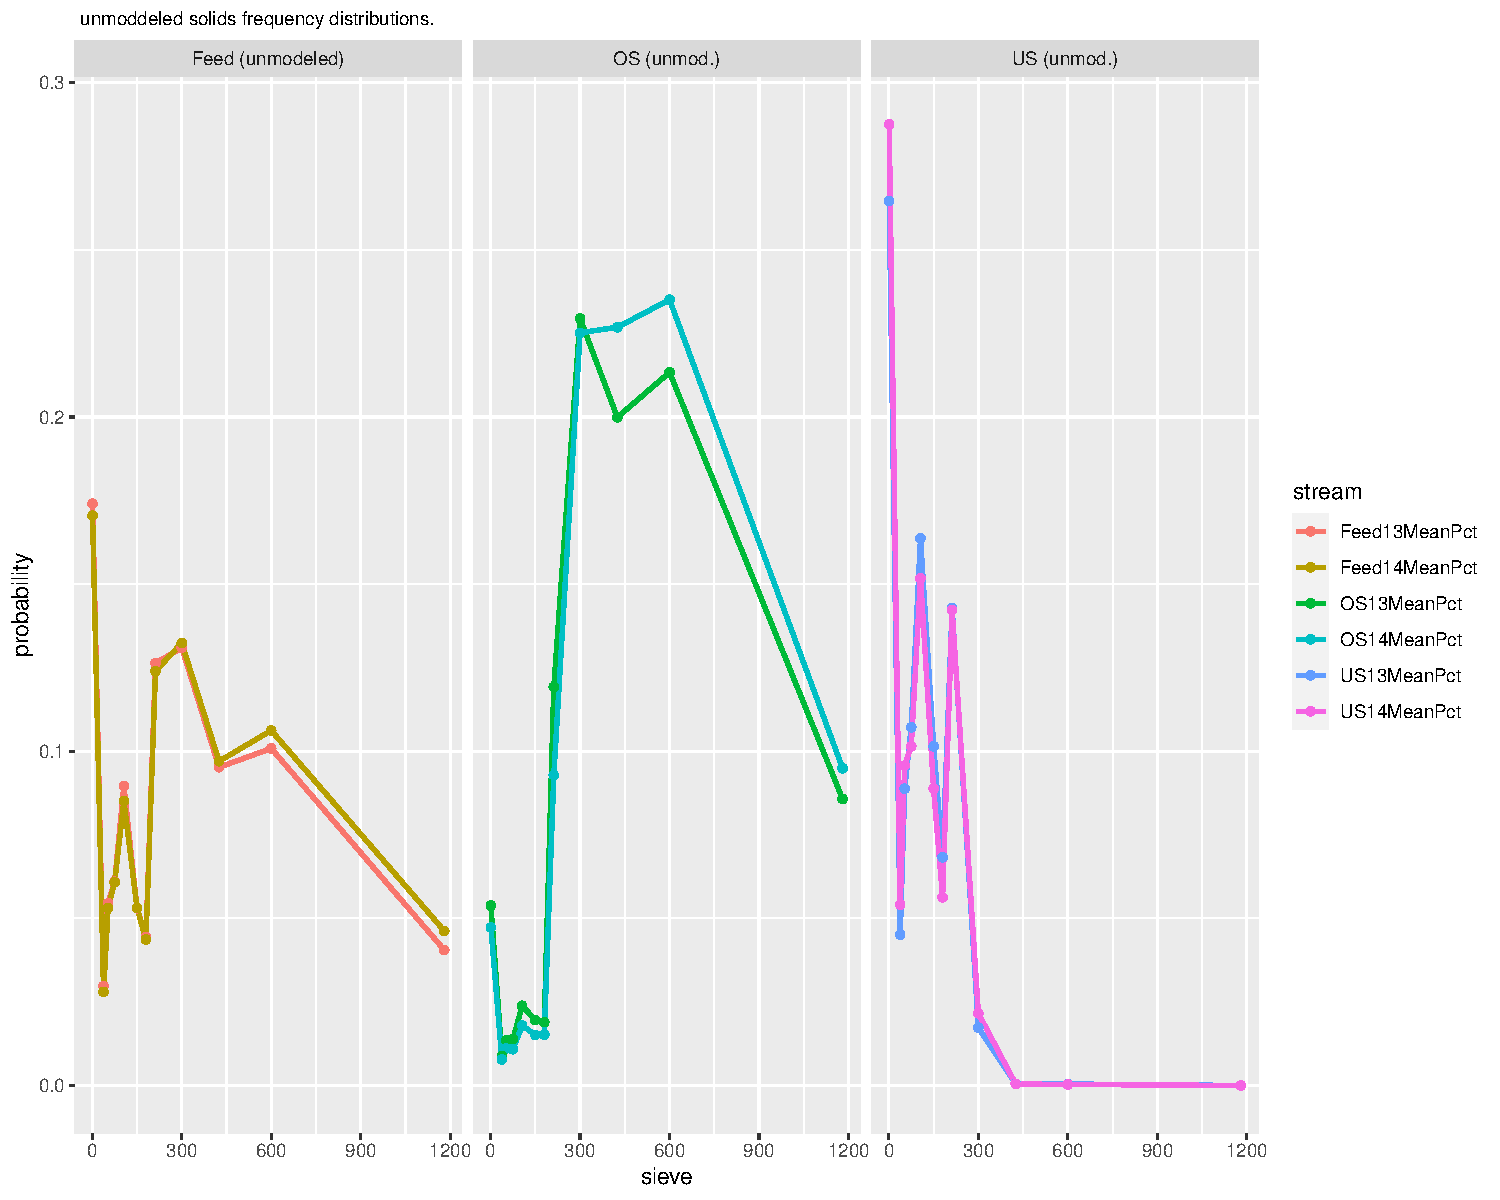
\includegraphics[width=0.5\linewidth]{C:/Users/miked/OneDrive/Statistics/R/Projects/nuiphao/2014-revisit-panelcomparison/05_fig_output/allStreamsPreModelling} 

}

\caption{Caption set from chunk options}\label{fig:unnamed-chunk-12}
\end{figure}

\begin{figure}

{\centering 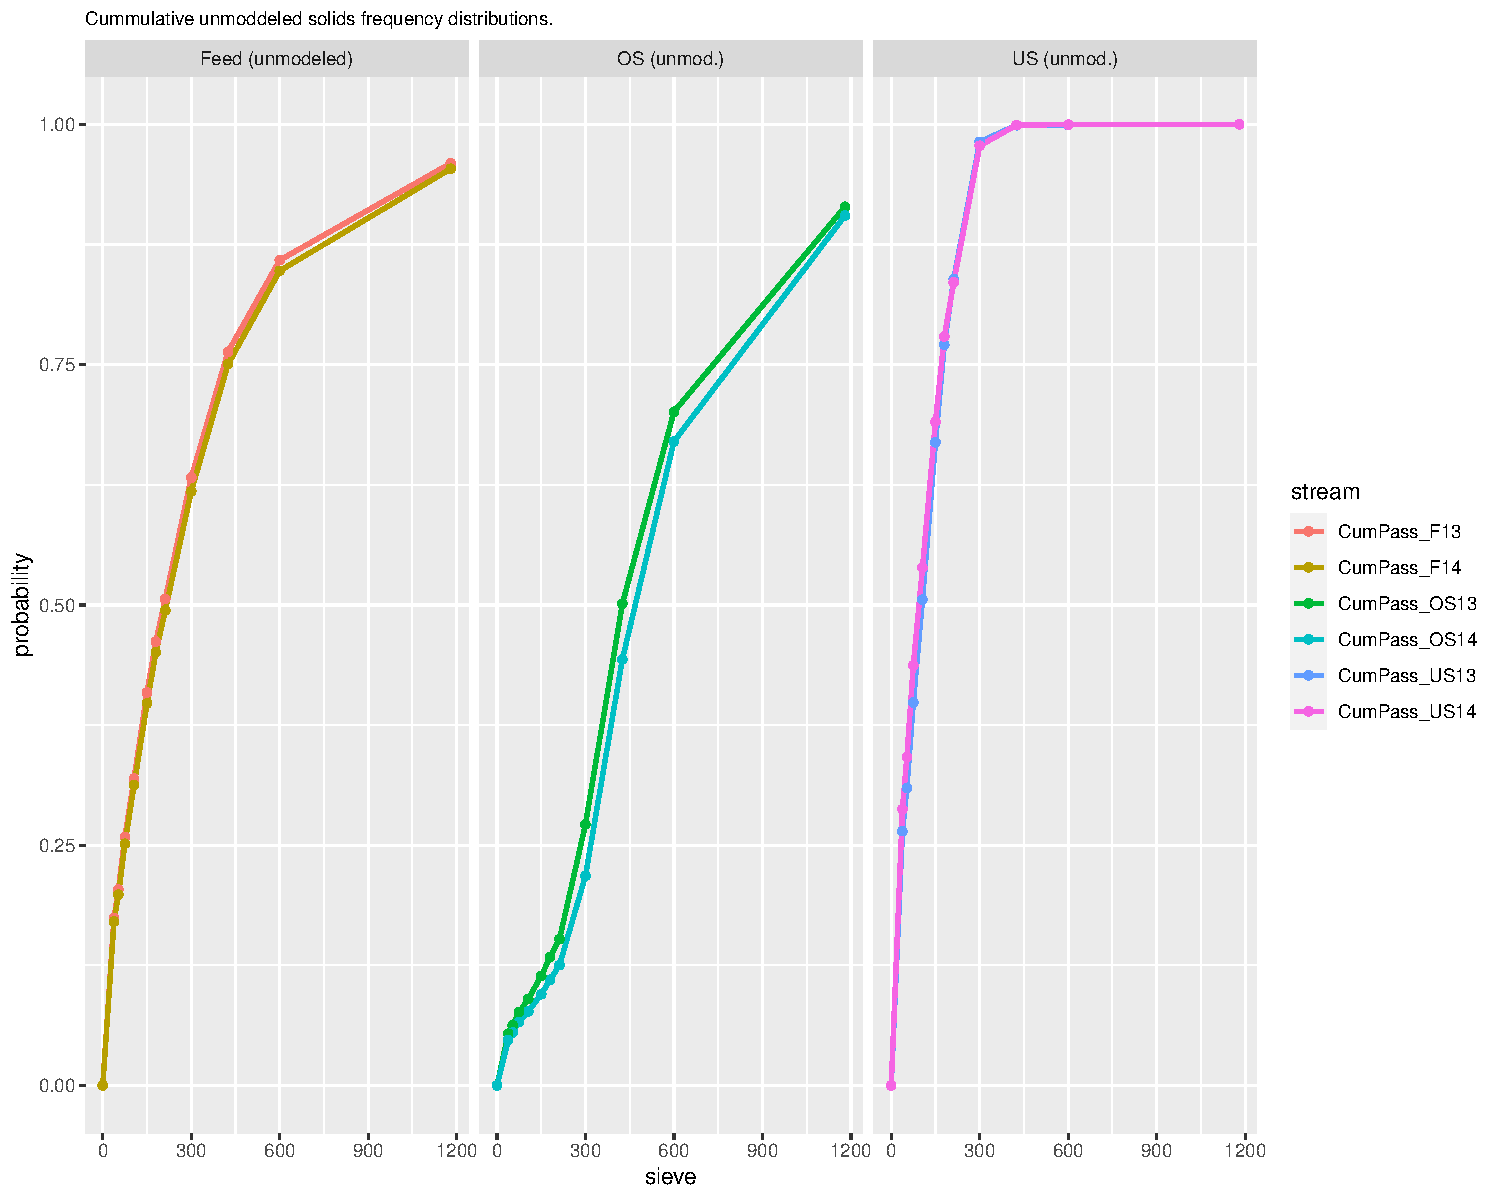
\includegraphics[width=0.6\linewidth]{C:/Users/miked/OneDrive/Statistics/R/Projects/nuiphao/2014-revisit-panelcomparison/05_fig_output/allStreamsCummulativePreModelling} 

}

\caption{Caption set from chunk options}\label{fig:unnamed-chunk-13}
\end{figure}

\begin{figure}

{\centering 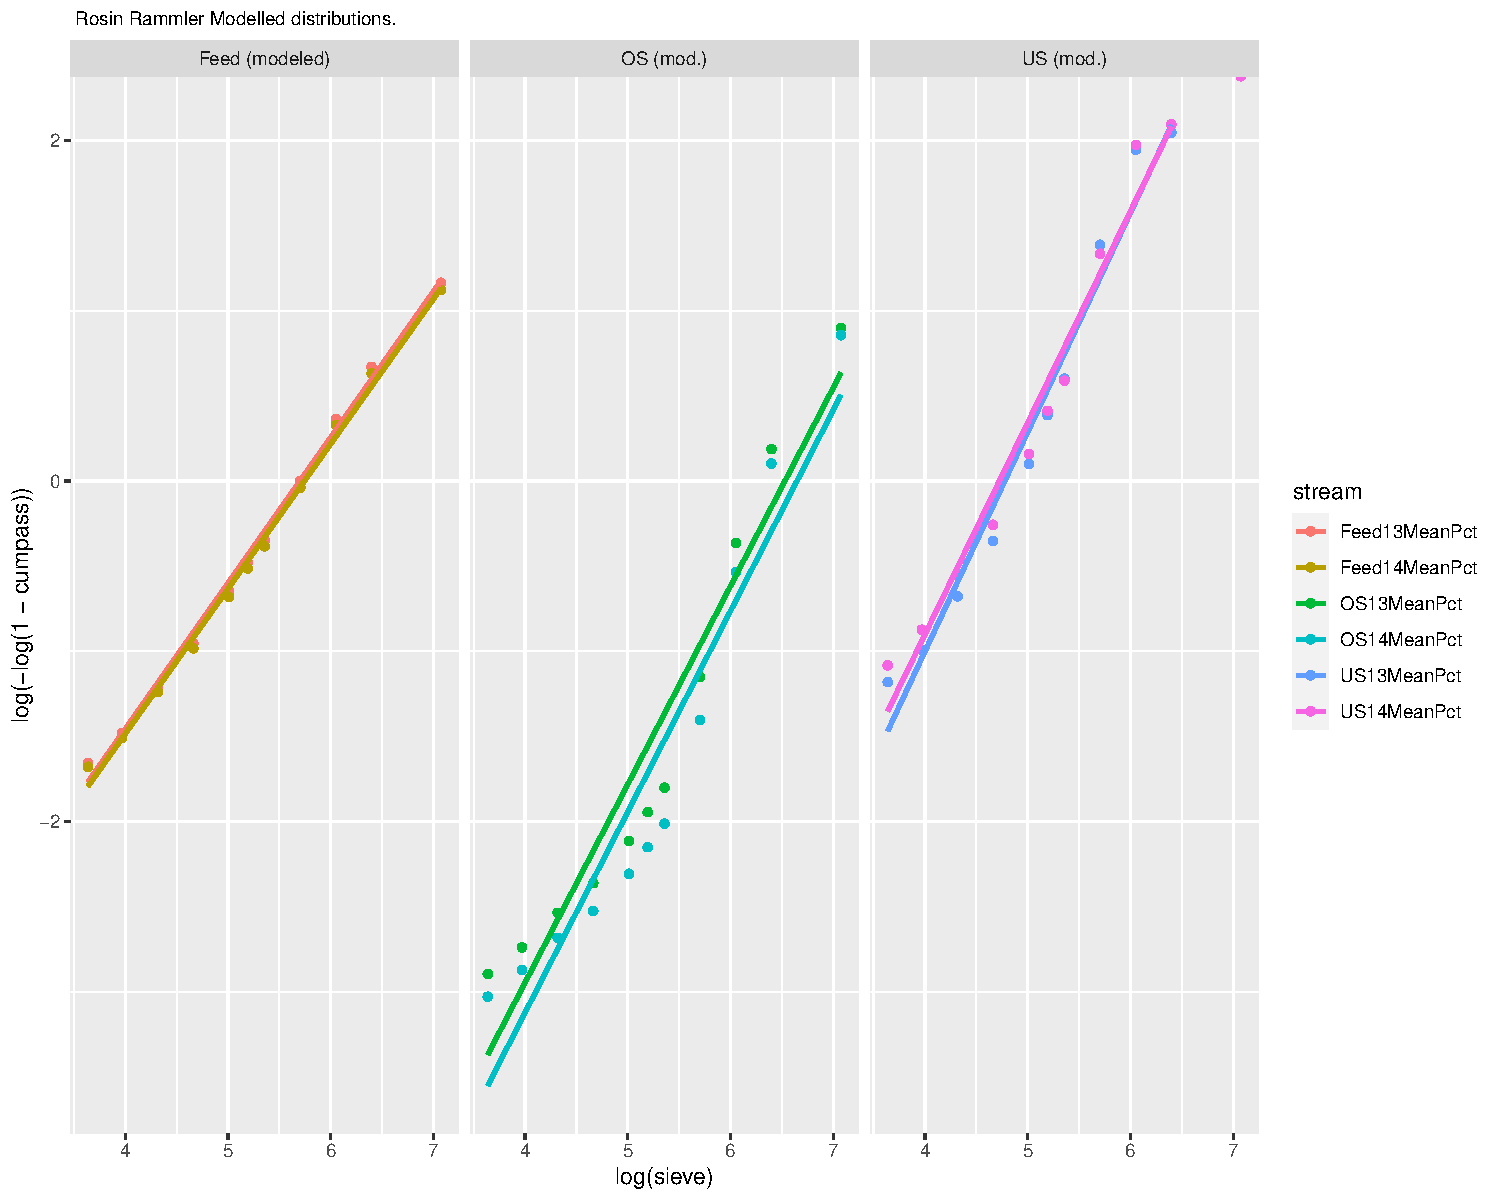
\includegraphics[width=0.6\linewidth]{C:/Users/miked/OneDrive/Statistics/R/Projects/nuiphao/2014-revisit-panelcomparison/05_fig_output/RRModelled} 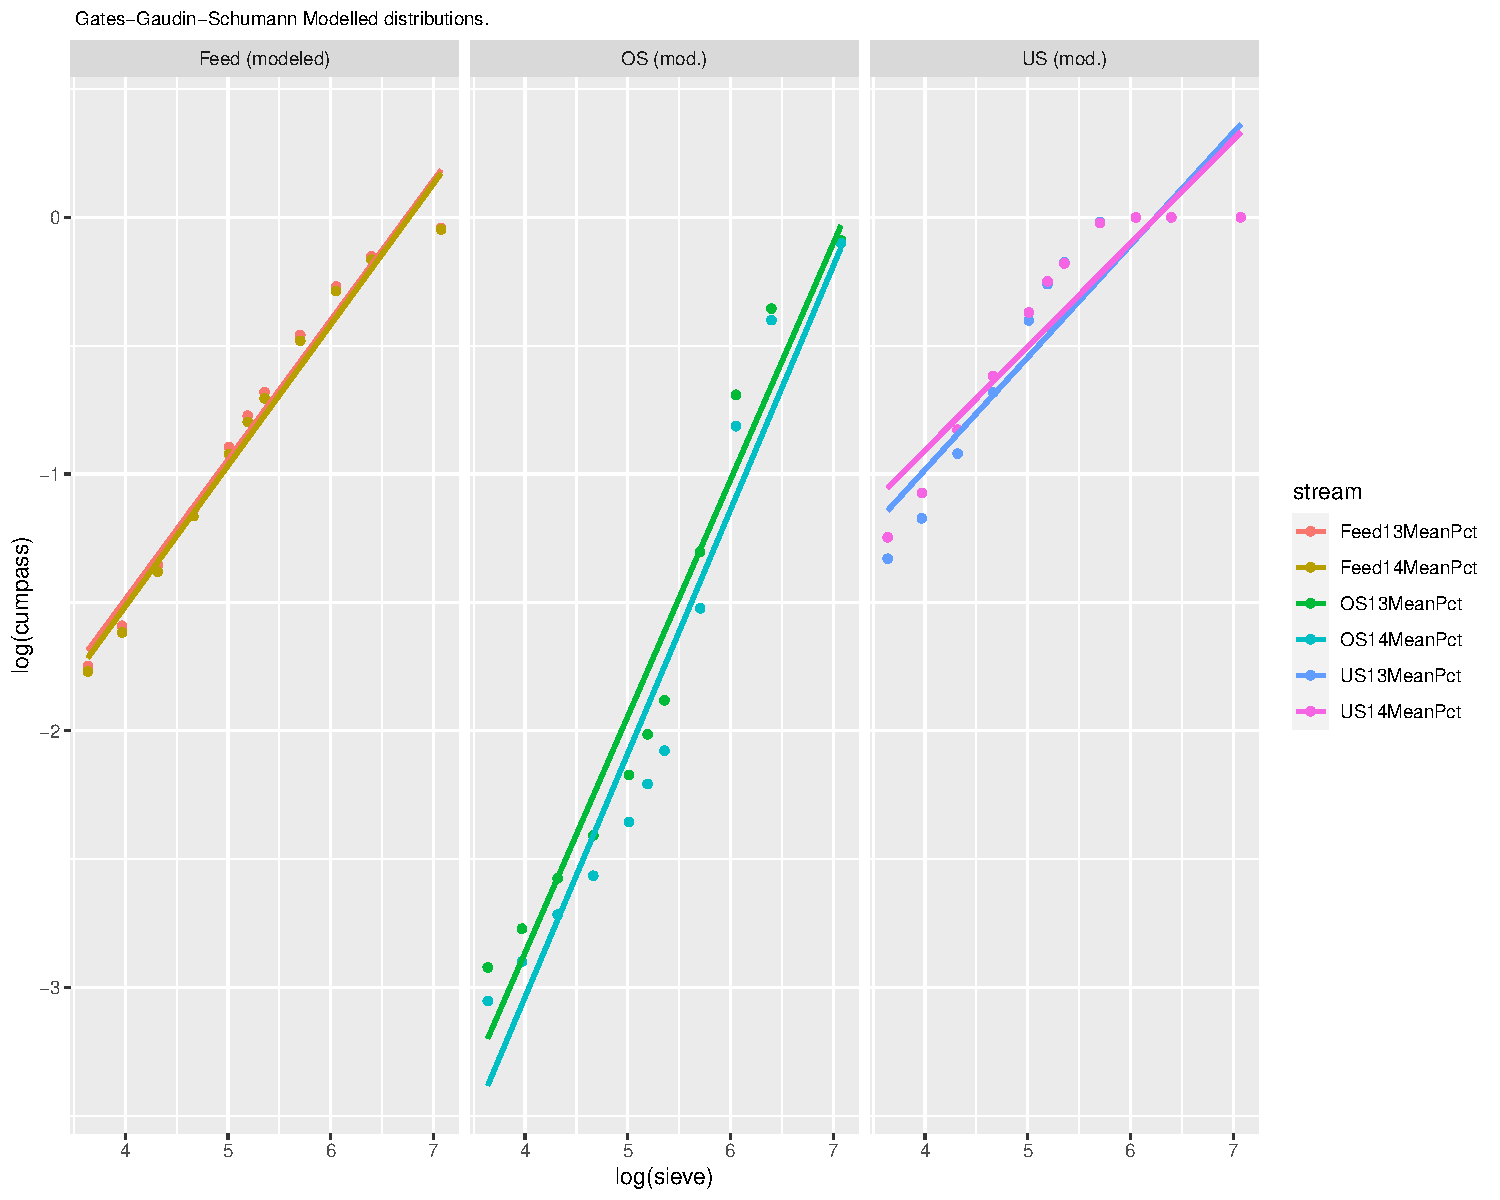
\includegraphics[width=0.6\linewidth]{C:/Users/miked/OneDrive/Statistics/R/Projects/nuiphao/2014-revisit-panelcomparison/05_fig_output/GGSModelled} 

}

\caption{Caption set from chunk options}\label{fig:unnamed-chunk-14}
\end{figure}

The two most commmonly used distributions in Geology and Mineral
Processing and specifically comminution circuits are the Roslin-Rammler
and the Gates-Gaudin-Schumann distributions.

Both models were used to model all PSD screening data to, and the
subsequent best fit model was selected in each case. Model selection was
determined by comparing each PSD's transformed linear model's
determinant (\(R^2\)).

RR model fits the feed streams means (Feed13Mean and Feed14Mean) better
(near straight line QQ fits) than the Oversize streams.

If the transformed size distributions from a crushing or grinding
operation do not approximate a straight line, it suggests that there may
have been a problem with the data collection, or there is something
unusual happening in the comminution process (hang-ups or unnuasual
recirculation). The size modulus is a measure of how coarse the size
distribution is, and the distribution modulus is a measure of how broad
the size distribution is. Size modulus for a size distribution can be
determined from a graph by extrapolating the straight-line portion up to
100\% passing and finding the corresponding size value. The distribution
modulus can be calculated by choosing two points in the linear portion
of the graph, calculating the logs of the sizes and \% passing values,
and calculating the slope.

Interpolation betweeen measured sizing points is conducted by the
back-transformation of the model-fitted points along the respective
model's distribution function.

try another approach for the R2 table: here brought in a s child
document. As the previous approach failed to save a readable image of
the table.

New child starts here..

Aim of this file: Generate table (r-saquared) for chapter (child) input
to base.Rmd (mother)

Reason: i cant get the table to gerate from within a code chunk or
r.script, but only once knitted does the table show.., so for now i 'll
keep it sepparate here in this (its own) .Rmd.

This file:

\begin{itemize}
\tightlist
\item
  reads code from: ``02\_rpackages'',`projectpackages.R' for libraries.
\item
  reads code from: ``03\_code/01\_code-output'',``R2RR.csv''
\item
  reads code from: ``03\_code/01\_code-output'',``R2GGS.csv''
\end{itemize}

and

\begin{itemize}
\tightlist
\item
  outputs code to: 05\_Results-and-discussion.Rmd
\end{itemize}

\begin{table}[!htb]
    \begin{minipage}{.5\linewidth}
      \caption{RR Model(formula)}
      \centering 
\begin{tabular}{>{\raggedright\arraybackslash}p{2.3cm}>{\raggedleft\arraybackslash}p{0.9cm}>{\raggedleft\arraybackslash}p{0.9cm}>{\raggedleft\arraybackslash}p{0.9cm}>{\raggedleft\arraybackslash}p{0.9cm}}
\toprule
stream & R2 & adj.R2 & p.value & AIC\\
\midrule
Feed13MeanPct & 0.996 & 0.995 & 0 & -26.0\\
Feed14MeanPct & 0.996 & 0.995 & 0 & -25.7\\
OS13MeanPct & 0.935 & 0.928 & 0 & 11.2\\
OS14MeanPct & 0.919 & 0.910 & 0 & 14.2\\
US13MeanPct & 0.979 & 0.977 & 0 & 1.4\\
\addlinespace
US14MeanPct & 0.978 & 0.975 & 0 & 1.6\\
\bottomrule
\end{tabular} \end{minipage}%
    \begin{minipage}{.5\linewidth}
      \centering
        \caption{GGS Model(formula)} 
\begin{tabular}{>{\raggedright\arraybackslash}p{2.3cm}>{\raggedleft\arraybackslash}p{0.9cm}>{\raggedleft\arraybackslash}p{0.9cm}>{\raggedleft\arraybackslash}p{0.9cm}>{\raggedleft\arraybackslash}p{0.9cm}}
\toprule
stream & R2 & adj.R2 & p.value & AIC\\
\midrule
Feed13MeanPct & 0.971 & 0.968 & 0e+00 & -14.8\\
Feed14MeanPct & 0.973 & 0.970 & 0e+00 & -15.5\\
OS13MeanPct & 0.951 & 0.946 & 0e+00 & 2.7\\
OS14MeanPct & 0.938 & 0.931 & 0e+00 & 6.2\\
US13MeanPct & 0.851 & 0.835 & 1e-04 & -0.2\\
\addlinespace
US14MeanPct & 0.855 & 0.839 & 0e+00 & -2.3\\
\bottomrule
\end{tabular} \end{minipage} 
\end{table}

and Ends here..

Another New New child starts here..

\begin{table}[!htb]
    \begin{minipage}{.5\linewidth}
      \caption{RR Model Coeficients}
      \centering \begin{table}[H]
\centering
\begin{tabular}{>{\raggedright\arraybackslash}p{3cm}>{\raggedright\arraybackslash}p{1.5cm}>{\raggedleft\arraybackslash}p{1.5cm}}
\toprule
stream & term & estimate\\
\midrule
Feed13MeanPct & (Intercept) & -4.884\\
Feed13MeanPct & log(sieve) & 0.857\\
Feed14MeanPct & (Intercept) & -4.891\\
Feed14MeanPct & log(sieve) & 0.852\\
OS13MeanPct & (Intercept) & -7.604\\
\addlinespace
OS13MeanPct & log(sieve) & 1.165\\
OS14MeanPct & (Intercept) & -7.841\\
OS14MeanPct & log(sieve) & 1.180\\
US13MeanPct & (Intercept) & -6.438\\
US13MeanPct & log(sieve) & 1.349\\
\addlinespace
US14MeanPct & (Intercept) & -6.188\\
US14MeanPct & log(sieve) & 1.311\\
\bottomrule
\end{tabular}
\end{table} \end{minipage}%
    \begin{minipage}{.5\linewidth}
      \centering
        \caption{GGS Model Coeficients} \begin{table}[H]
\centering
\begin{tabular}{>{\raggedright\arraybackslash}p{3cm}>{\raggedright\arraybackslash}p{1.5cm}>{\raggedleft\arraybackslash}p{1.5cm}}
\toprule
stream & term & estimate\\
\midrule
Feed13MeanPct & (Intercept) & -3.667\\
Feed13MeanPct & log(sieve) & 0.544\\
Feed14MeanPct & (Intercept) & -3.713\\
Feed14MeanPct & log(sieve) & 0.549\\
OS13MeanPct & (Intercept) & -6.549\\
\addlinespace
OS13MeanPct & log(sieve) & 0.921\\
OS14MeanPct & (Intercept) & -6.835\\
OS14MeanPct & log(sieve) & 0.950\\
US13MeanPct & (Intercept) & -2.735\\
US13MeanPct & log(sieve) & 0.438\\
\addlinespace
US14MeanPct & (Intercept) & -2.520\\
US14MeanPct & log(sieve) & 0.403\\
\bottomrule
\end{tabular}
\end{table} \end{minipage}
\end{table}

and Ends here..

try add as footnote in table/s: "RRmodel is a better fit ,according to
the simple model applied, i.e.~single linear model applied to
transformed y-variables and transformed x-factors. When applyinh
peicewise (conditional) factors, the GGS model becomes a better model,
but at the same tiem more noise (errors (epsilon?) is incorpaorated in
the model. double the coefficients.

\hypertarget{to-do}{%
\section{To Do}\label{to-do}}

Include instructions (steps) on which files to Run of Knit to preduce
the final report.

fix output location of knits for files in /04-text

\begin{itemize}
\tightlist
\item
  make a subfolder (output)
\end{itemize}

draw diagram that outlines workflow of this project\ldots draw data in
then munge then write to table to\ldots, then import data from to
.rmd\ldots bla bla

Remove typos! Use the devtools::spell\_check() function. Typos in
documentation are not the end of the world but can annoy the user, and
it's not hard to remove them thanks to this tool, so do it when you get
a chance.

lots of advice to follow here

\url{https://holtzy.github.io/Pimp-my-rmd/}

\url{https://cran.r-project.org/web/packages/kableExtra/vignettes/awesome_table_in_html.html}

\hypertarget{data}{%
\subsection{Data}\label{data}}

\hypertarget{write-up}{%
\subsection{Write up}\label{write-up}}

explain and list the test that were conducted. explain which part are
taken further into considerring for analasys and why.

Im not too happy with the layout structure and flow. compare with
professional technical report in the industry.

\hypertarget{tables-plot-figs-formulas}{%
\subsection{Tables, Plot, Figs,
Formulas}\label{tables-plot-figs-formulas}}

\hypertarget{plot}{%
\subsubsection{Plot}\label{plot}}

simple small plots off all raw distributions.

this same plot can be plot next to the OS and US streams.

Then do the same for the modelled streams.

\hypertarget{formulas}{%
\subsubsection{Formulas}\label{formulas}}

\begin{itemize}
\tightlist
\item
  double check RR Latex formula in (d/l?)
\end{itemize}

\[F\left(d\right) = exp\left[-(\frac{d}{l})^{m} \right]\]

\begin{itemize}
\item
  add regression formulas that include the coeficients
\item
  result, discussion section?
\end{itemize}

\hypertarget{tables}{%
\subsubsection{Tables}\label{tables}}

\begin{itemize}
\item
  add row in distribution figures
\item
  wrap text in col names of R2
  tableshttps://community.rstudio.com/t/wrap-column-name-in-pdf-table-from-knitr-kable/3278/4
  +also add latex formulas
\item
  repair layout of model coef tables in "Results and Discussion sectio:
\item
  fix rounding
\item
  fix layout
\end{itemize}

The RR transformation is achieved by taking the natural log twice and
simplified as:
\#\[\ln\left\{-\ln\left[1-F(d)\right] \right\} = m\times \ln d - m\times \ln \bar{d} \]

\end{document}
